\documentclass[11pt,a4paper]{article}
\usepackage[vmargin=3cm, hmargin=3cm]{geometry}
\usepackage[utf8]{inputenc}
\usepackage{graphicx}
\usepackage{amsmath}
\newcommand{\argmax}[1]{\underset{#1}{\operatorname{arg}\operatorname{max}}\;}
\author{Frank Smit \& Sander Latour}
\title{A game of politics}
\begin{document}
\maketitle

\section{Introduction}
This work introduces and describes the game, `a game of politics'. In this game, the player plays the lead character who invented a super computer which enables him to control the mind of a leader during the prehistoric era. During that time, the power is all divided over different families. These different families have certain ideals and will request the leader for favors which will bring them closer of achieving those. In every turn, the player is able to approve one of these requests. Each request has is own consequences (positive or negative), and chosen consequences will influence the relationship between the families and the leader depending on their opinion about the made decision.

Credits are assigned to the player after each turn. The goal of the player is to earn as many credits as possible. The duration of the game in which the player receives credits is determined by the actions he takes. Therefore the player should carefully select his actions and think about the consequences it has for his own benefit.  

\section{Game}
\subsection{Game mechanics}
The game is a Turn-Based-Strategy (TBS) game, without any time restrictions in each turn. Thus the player has plenty of time to think about the strategy he will play. In every turn there are $N$ actions (from $N$ families) to choose from. These actions have effects, both negative and positive, to several topics of the world (such as food and safety).  After selecting an action, the agents will immediately react emotionally which causes change in their support. This will be positively if you protect the ideals of the agent and negatively otherwise. The support of the family is important to the player because after every turn, the the player needs to satisfy at least 60\% of the people. If the support is below this threshold, the people will stand up to you and start a revolution. The player then has three turns to get enough support before the game is finished.

When the player chooses sides and favors one action over the others there will be families that have gained and families that have lost. Since people tend to join the winning team there is a chance that some people will move from the losing family to the winning family. The more people that are represented by one family, the more people you can make happy by approving that family's request. When a family is completely satisfied with your policy, they could decide to support you unconditionally. This means that they will support you completely and will not ask for any favors in return. However, they will still look over your shoulder and they still react emotionally to the chosen actions. This means that you must remember to protect the interests of the families that are not explicitly asking anything themselves, because if you don't they will loose their belief in you.

The way the player creates support greatly influences the duration of the game and the final credit score that is achieved. The player could try to make almost everybody happy by in turn approve one of their requests. This usually results in a long period of just enough support to keep playing, but tends to have less risk since nobody is really held back. The player could also slowly shift the power towards fewer families to concentrate the support by favoring them more than others. This should however not happen too quickly since the other families could then react so severely that a revolution brakes out. However, this strategy usually results in much higher support which will enable the player to favor himself over the families and buy more credits. Caution is advised though, since the families will not appreciate this. And concentrating the support also means that you can loose it more quickly.

Once the player looses too much support or retires after 65 steps, the game ends and the credits that were gathered are shown. This creates a motivation to play again to improve your score. The credits metric also makes the result comparable to strategies of your friends.
\subsection{Game situations}

  \subsubsection{The winner takes it all}
Every action in every turn leads to some families that won that round and some families that lost that round. This is determined by calculating how much, trough the families' eyes, the world was made better after selecting that action. In other words, the consequences of the action are weighted according to the ideals of a family. The family that gained the most is considered the winner and the family that gained the least is considered the loser. 

As mentioned above, the families could become more powerful after selecting some actions. This is done using the winner and losers concept, where some amount of power from the  family that lost is transferred to the family that won. This can be seen as people renegade from one family to the other family. The amount of power that is transferred is determined by following this list of steps.
\begin{enumerate}
  \item Let $r$ denote a random number between 0 and 1.
  \item Let $c_s$ denote a shifting constant describing the rate of power change (in the implementation this is set to 0.1)
  \item Let $\delta_w$ denote the weighted gain the winner has achieved.
  \item Let $\delta_l$ denote the weighted loss the loser has achieved.
  \item Let $P_w$ denote the amount of power (i.e. amount of people) of the winning family.
  \item Ley $P_l$ denote the amount of power of the losing family.
  \item Let $p$ denote $\frac{(100 - \lvert P_w - P_l \rvert)}{100}$
  \item Return $r c_s p \lvert \delta_l - \delta_w \rvert$
\end{enumerate}

\subsubsection{Revolution}
When the player has less than 60\% of the support, a revolution brakes out. This means that the people grant the player with three turns to rewin their support. If at the end of those three turns the support is still too low, the player has to resign and the game ends. Thoughts have arose to make the families desire more during the revolution due to their unhappiness, but this was not included in the final implementation.

\subsubsection{Retirement}
After 65 turns, the leader will decide to retire from his function. Once this happens the player has lead the leader to a successful reign and will be rewarded for his service record. This reward will be in terms of extra credits. 

\subsection{Music}
Music is added to the game to enhance the gaming experience. There are two different states in the game that alters the music. The first one is the normal situation where the player is just picking actions and the agents are reacting to the actions. The second one is when the support is below the threshold of 60\%, i.e. when the revolution starts. The music then is changed to a more tension increasing piece of music. This will create more excitement for the player, knowing that he will need to watch his steps. 

\section{Implementation details}
  \subsection{World state}
    Actions that are performed have an effect on the world. These effects are in turn used by other agents to determine their reaction on the performed action. Since actions can have both positive and negative effects they can reverse some of the earlier actions taken in terms of the world state. To avoid the enormous complexity of a set of boolean variables to represent the diversity of actions and cater for the reversal effect like one would in a classical STRIPS approach, we instead chose to represent the world in a $n$-dimensional space of $n$ real-valued topics. These topics represent typical themes that have been playing a role in politics for a long time. The topics that we have used for the current implementation are \emph{food}, \emph{safety} and \emph{culture}. This list is however extendable. Each world state consist of $n$ topic-value pairs representing the current state of each topic in that world state.
  \subsection{Actions}
    Not unlike STRIPS actions consist of two parts, a condition and the effect. These two components are described in terms of the topic space as was discussed earlier.
    \subsubsection{Conditions}
      Each action has a set of topic-value pairs that represents the minimum value that each mentioned topic must have in the world state before the action is requested. This is motivated by the following reasoning. If an agent values a specific topic it will naturally try to improve that topic as much as possible. However if the basic necessities of a topic are not arranged yet, it has no use to request higher level improvements since they typically rely on the presence of more basic improvements for their effectiveness. The topic values for consecutive actions are increasing. The condition also has the effect that when another action decreases a topic value, it might result in some agent requesting earlier actions again.
    \subsubsection{Effects}
      Each action has a set of topic-value pairs that represents the effect it has on the world state. The values can be both positive and negative indicating positive and negative effects respectively. The new world state can be determined by simply adding each of the effect values to the current world state values.
  \subsection{Autonomous agents}
    Most players in the game are autonomous agents that each turn determine which action they would most desire to see executed by the human player. This desire is expressed to the human player at the beginning of each turn. When a human player decides which action to execute, each autonomous agent will determine his reaction to this action. The reaction is a positive or negative change in their emotional state.
    \subsubsection{Selecting desired action}
      Each agent selects their next desired action according to the following list of steps.
      \begin{enumerate}
        \item Let $\vec{s}$ denote a real-valued vector, where each element denotes the value of a topic in the current world state.
        \item Let $a$ denote an action, consisting of a condition component denoted as $a_C$ and an effect component denoted as $a_E$.
        \item Let $\mathcal{A}$ denote the set of all actions, such that for each valid action $a$ it holds that $a \in \mathcal{A}$.
        \item Let \textsc{Performable}($a_C$,$\vec{s}$) denote a boolean function that returns true when every condition in $a_C$ is met in world state $\vec{s}$.
        \item Let $\mathcal{P}$ denote the set \{\textsc{Performable}($x$)$\vert x \in \mathcal{A}$\}.
        \item Let $\vec{w}$ denote a real-valued vector, where each element denotes the weight of a topic in the world state indicating the preference of the agent.

        \item Return $\argmax{a \in \mathcal{P}} \left[ a_E \cdot \vec{w} \right]$.
      \end{enumerate}
    \subsubsection{Preferences}
      Each autonomous agent prefers improvement in some topics more than in others. It might even prefer to worsen the situation of a specific topic. This is expressed in the preferences, which is a set of topic-weight pairs where the weights adds up to 1. These weights indicate how much they value improvement on that topic.
    \subsubsection{Emotion states}
    \begin{figure}
\centering
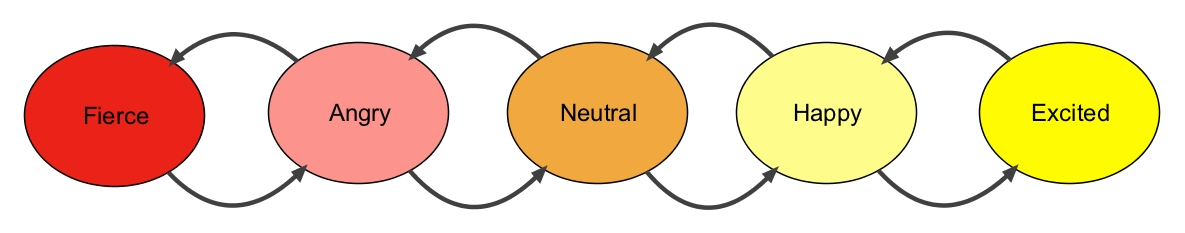
\includegraphics[scale=0.25]{States-image}
\caption{The emotional states.}
\label{fig:es}
\end{figure}
      Each autonomous agent has a certain amount of emotional energy. This energy is increased when the agent is more pleased. After each turn agents update their emotional energy by summing up the multiplication of the preference weights with the effects of the taken action, which results in the delta value that is added to the current emotional energy level. The continuous domain of the energy is discretized in a FSM of emotional states shown in figure \ref{fig:es}. The transitions in this FSM are absolute energy values that the agent must be in to switch to a different emotion state. For example, given a sufficiently large negative value an agent will transition from a neutral to an anger state. The current implementation does not use these emotion states very extensively, besides using them to make the energy values more intuitive to understand for the human player. However, they cater for complex behavior where each agent may behave differently in a different emotion state.

  \subsection{Human agent}
        \begin{figure}[h!]
      \centering
      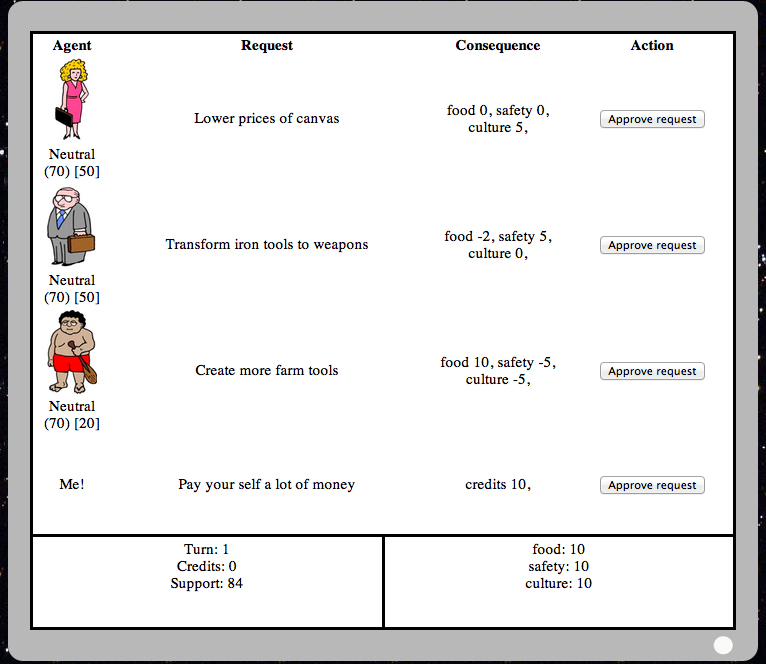
\includegraphics[scale=0.45]{screenshot}
      \caption{A screenshot of the game. The interface is simple and intuitive, having different screens containing different types of information. }
      \label{fig:scr}
      \end{figure}
      
    \subsubsection{Interface}
      The interface of the game, as shown by figure \ref{fig:scr}, is extremely simple and intuitive. Because the story of the game allows the player to play as a scientist who created a super computer, the only screen the player will look at is a computer screen. This screen contains three areas. The first area is the largest one, where the agents together with their request and the consequences are presented. At each line the player has the ability to press the `Approve request' button. This button represents the action the player could take. 

      In the small area left below in the screen, the game information is presented to the player. Here information such as, in which turn the player is, how much credits it received so far, and how much support the player has from the agents. This information will be updated after every turn. In the small area in the right corner below, the world state is presented to the player. This shows the current values of the topics that together form the world state. These topics are the same as the consequences of each action. 

  \subsection{Game loop}
      The game controller proceeds through various phases each turn, as shown in figure \ref{fig:gl}. At the end of the fourth phase the cycle starts over. These four cycles will be explained in the next sections. 
      
  \begin{figure}[h!]
  \centering
	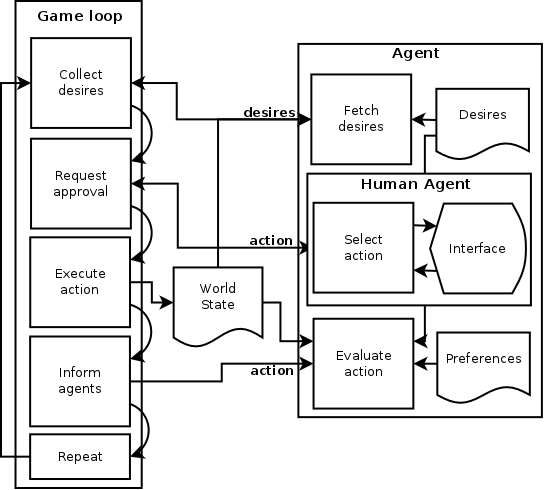
\includegraphics[scale=0.25]{gameloop.png}
	\caption{The game loop with all its components.}
	\label{fig:gl}  
  \end{figure}
 
    \subsubsection{Collect desires}
      In the first phase the game controller requests the autonomous agents to express their desired actions based on the current world state.
    \subsubsection{Request approval}
      In the second phase the game controller communicates these desired actions to the human player and requests him to approve one of the actions.
    \subsubsection{Execute action}
      The approved action is executed in the third phase by adding the effects of the action to the current world state.
    \subsubsection{Inform agents}
      The new world state is communicated to autonomous agents in the fourth phase. Each agent in turn will update their emotional energy. 

\section{Conclusion}
A game of politics can be considered as a serious game that simulates a part of the decision making process of leaders in a small domain. Multiple strategies can be executed to reach the goal, although it is not clear whether all strategies have equal chances. The counter players are autonomous agents that respond to the actions of the human player. The gathering of credits and the situation-dependent music create a more engaging game experience.

\section{Reflection}
Creating a good game with a good gameplay is a very difficult task. We have learned a lot from building this game and thinking about how the game should develop in certain circumstances. For example, it turned out to be very hard to balance the realism of the game with what can be created in practice. We wanted, for example, to create a whole economy which is influenced by decisions that the player makes, but at the same time limits the possibilities of the player. However, modeling the economy was much too complex for both the developers as for the human player to understand how to deal with that. During the development of this game, various dilemmas focused on realism were encountered. 

We aimed for good gameplay with very intelligent agents, so we thought about various factors to (give the impression of) complex behavior. The difficult part however is to create such intelligent agents and still keep them understandable for the player. Modeling an autonomous agent is fun, if and only if you have a good change of succeeding in that. We considered quite a lot of AI techniques and data representations to achieve this, such as GOAP, STRIPS, behavioral trees, etc. Eventually we took a slightly more computer science approach which still lead to the impression of intelligent behavior, without some of the enormous engineering tasks of creating action ontologies in order to make it realistic.

It also became clear that the story element in a game is an important factor. It also appeared to be non-trivial to construct that story around all the game elements that were designed during brainstorm sessions. Especially when combining this with the point about realism.

We did not want the game to be very straightforward or that one strategy would outperform other strategies. Therefore we really had to think about how to make the game interesting for different strategies, and how we could alter the gameplay such that this was the case.

In the end we managed to create a working and partially engaging game, but quite some obstacles had to be dealt with in the process.
\end{document}
